%!TEX program = xelatex
%!BIB program = bibtex
\documentclass[a4paper,zihao=-4]{article}
\usepackage[UTF8,punct,linespread=1.56]{ctex}
% \documentclass[a4paper,cs4size,UTF8,punct,linespread=1.56]{ctexart}
\pagestyle{empty} % 第二页以后页码空白
\usepackage[a4paper, left = 3.2cm, right = 3.2cm, top = 2.54cm, bottom = 2.54cm]{geometry}
\usepackage{xcolor}
% \usepackage[citebordercolor = white]{hyperref}
\usepackage[hidelinks]{hyperref}
\usepackage{graphicx}
\usepackage{amsmath}
\usepackage{amssymb}
\usepackage{times}
\usepackage[subrefformat=parens,labelformat=parens]{subfig} %
\usepackage{booktabs} % for \toprule \midrule \bottomrule \cmidrule
\usepackage{cleveref}
\crefformat{table}{表~#2#1#3}
\crefformat{figure}{图~#2#1#3}
\crefformat{equation}{式~(#2#1#3)}
\usepackage{enumitem}
% \setenumerate[1]{itemsep = 0pt, parsep = 0pt, topsep = 2bp}
\setlist[enumerate]{itemsep = 0pt, parsep = 0pt, topsep = 2bp}
% \setitemize[1]{itemsep = 0pt, parsep = 0pt, topsep = 2bp}
\setlist[itemize]{itemsep = 0pt, parsep = 0pt, topsep = 2bp}
\usepackage{fontspec}
\setmainfont{Times New Roman}
% \usepackage{minted}   % For syntax highlighting
% \usemintedstyle{friendly}
\usepackage{setspace}
\usepackage{caption}
% \usepackage{multibib}
% \newcites{extra}{补充参考资料}%  \citelatex, \nocitelatex, ...

% \usepackage[strings]{underscore} #workaround for underscore in DOI; fixed

% \DeclareCaptionFont{capfont}{\kaishu\zihao{-4}\selectfont} % Caption font
% \DeclareCaptionFont{subfont}{\kaishu\zihao{5}\selectfont} % Sub-caption font
% \captionsetup{font = capfont}
% \captionsetup[subfigure]{font = subfont}
\captionsetup[figure]{labelsep=space} % 空格 space;点 period;冒号 colon
\captionsetup[table]{labelsep=space}  % 空格 space;点 period;冒号 colon

\usepackage{titlesec}
\titleformat{\subsubsection}[block]{\hspace{3em}}{\thesubsubsection}{1em}{}
\graphicspath{{images/}}   % 设置图片所存放的目录
\usepackage{insfc}
% \usepackage[square,numbers,sort&compress]{natbib}   % replaced with gbt7714
\usepackage[authoryear]{gbt7714}
\newcommand{\citess}[1]{\textsuperscript{\cite{#1}}}
\setlength{\bibsep}{1pt plus 0.3ex}

\begin{document}

% \kaishu

% Decrease space above and below equations
\setlength{\abovedisplayskip}{0pt}
\setlength{\belowdisplayskip}{0pt}

%%%%%%%%% TITLE %%%%%%%%%
% \title{报告正文 \vspace{-3.4ex}}
% \title{报告正文}
% \maketitle
\thispagestyle{empty}    % 首页页码空白

\vspace*{-23pt} %调整 报告正文 文字与上边缘的距离
\begin{center}
  {\kaishu \zihao{3} \textbf{报告正文} }
\end{center}

%%%%%%%%% Your Content %%%%%%%%%
\vspace{-5pt} % 调整 报告正文 文字与正文的距离
{\kaishu \zihao{4} 参照以下提纲撰写,要求内容翔实、清晰,层次分明,标题突出。}\alert{请勿删除或改动下述提纲标题及括号中的文字。\vspace{9bp}}

\NsfcChapter{(一)立项依据与研究内容}{(建议8000字以内):}

\NsfcSection{1}{项目的立项依据}{(研究意义、国内外研究现状及发展动态分析,需结合科学研究发展趋势来论述科学意义;或结合国民经济和社会发展中迫切需要解决的关键科技问题来论述其应用前景。附主要参考文献目录);}

研究意义、
国内外研究现状及发展动态分析、
科学意义或应用前景
\citep{Einstein1905AnP}。

% \begin{figure}[!htb]
%   \centering
%   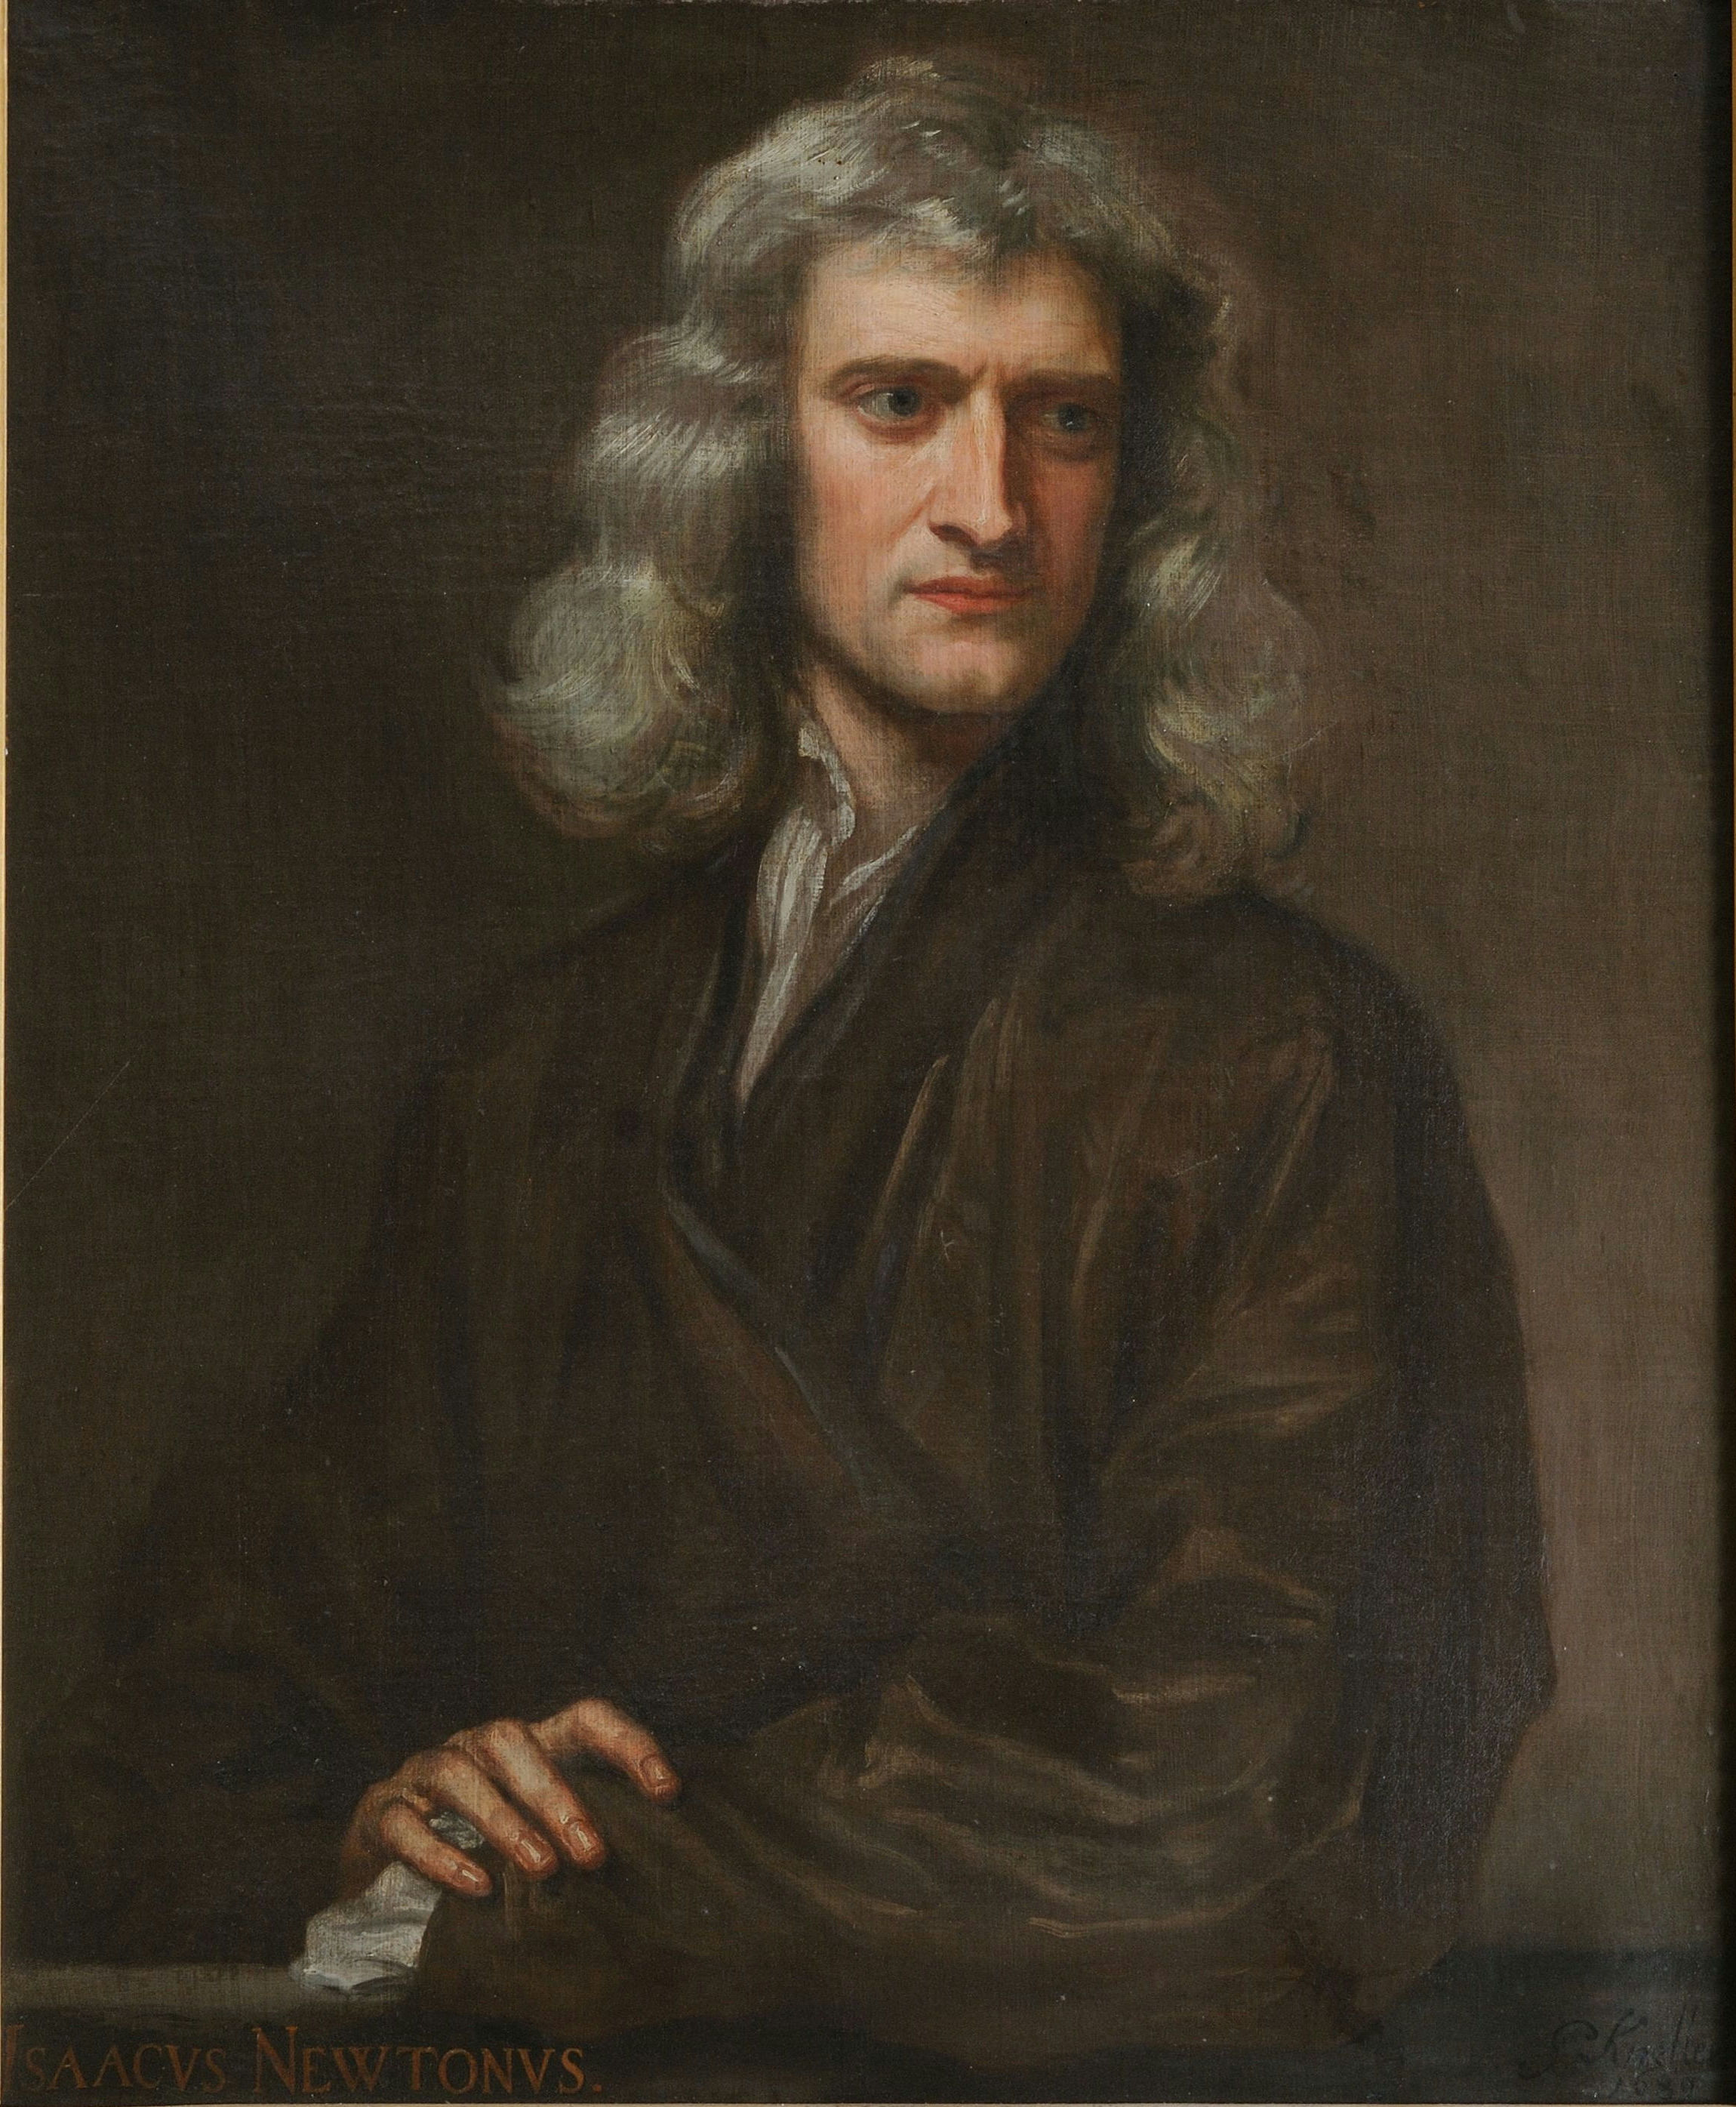
\includegraphics[scale=0.05]{Newton.jpg}
%   \caption{祝你好运!}
%   \end{figure}


\begin{spacing}{1.3} % 行距
	\zihao{5} \songti
  \bibliography{ref}
	\vspace{11bp}
\end{spacing}

\smallbreak
\NsfcSection{2}{项目的研究内容、研究目标,以及拟解决的关键科学问题}{(此部分为重点阐述内容);}
\subsection{研究内容}

\subsection{研究目标}

\subsection{拟解决的关键科学问题}


\smallbreak
\NsfcSection{3}{拟采取的研究方案及可行性分析}{(包括研究方法、技术路线、实验手段、关键技术等说明);}
\subsection{研究方案}\label{fangan}

\subsection{可行性分析}


\smallbreak
\NsfcSection{4}{本项目的特色与创新之处;}{}


\smallbreak
\NsfcSection{5}{年度研究计划及预期研究结果}{(包括拟组织的重要学术交流活动、国际合作与交流计划等)。}

\subsection{年度研究计划}

\subsection{预期研究结果}


\smallbreak
%%%%%%%%%%%%%%%%%%%%%%%%%%%%%%%%%%%%%%%%%%%%%%%%%
\NsfcChapter{(二)研究基础与工作条件}{}

\NsfcSection{1}{研究基础}{(与本项目相关的研究工作积累和已取得的研究工作成绩);}


\smallbreak
\NsfcSection{2}{工作条件}{(包括已具备的实验条件,尚缺少的实验条件和拟解决的途径,包括利用国家实验室、国家重点实验室和部门重点实验室等研究基地的计划与落实情况);}


\smallbreak
\NsfcSection{3}{正在承担的与本项目相关的科研项目情况}{(申请人正在承担的与本项目相关的科研项目情况,包括国家自然科学基金的项目和国家其他科技计划项目,要注明项目的名称和编号、经费来源、起止年月、与本项目的关系及负责的内容等);}


\smallbreak
\NsfcSection{4}{完成国家自然科学基金项目情况}{(对申请人负责的前一个已结题科学基金项目(项目名称及批准号)完成情况、后续研究进展及与本申请项目的关系加以详细说明。另附该已结题项目研究工作总结摘要(限500字)和相关成果的详细目录)。}


\smallbreak
%%%%%%%%%%%%%%%%%%%%%%%%%%%%%%%%%%%%%%%%%%%%%%%%%

\NsfcChapter{(三)其他需要说明的问题}{}


\NsfcSection{1}{}{申请人同年申请不同类型的国家自然科学基金项目情况(列明同年申请的其他项目的项目类型、项目名称信息,并说明与本项目之间的区别与联系)。}


\smallbreak
\NsfcSection{2}{}{具有高级专业技术职务(职称)的申请人是否存在同年申请或者参与申请国家自然科学基金项目的单位不一致的情况;如存在上述情况,列明所涉及人员的姓名,申请或参与申请的其他项目的项目类型、项目名称、单位名称、上述人员在该项目中是申请人还是参与者,并说明单位不一致原因。}


\smallbreak
\NsfcSection{3}{}{具有高级专业技术职务(职称)的申请人是否存在与正在承担的国家自然科学基金项目的单位不一致的情况;如存在上述情况,列明所涉及人员的姓名,正在承担项目的批准号、项目类型、项目名称、单位名称、起止年月,并说明单位不一致原因。}


\smallbreak
\NsfcSection{4}{}{其他。}


\end{document}
